\begin{problem}
  Circle \textbf{T} for \textit{true} or \textbf{F} for \textit{false}. (You
  don't need to justify your answers.)

  \begin{center}
    \begin{tabular}{lllp{0.6\linewidth}}
      \textbf{a.} & \textbf{T} & \textbf{F} & $\sin^{-1} (\sin (\frac{2\pi}{3})) = \frac{2\pi}{3}$ \\
      \textbf{b.} & \textbf{T} & \textbf{F} & $\cos (-t) = \cos (t)$ for all $t$. \\
      \textbf{c.} & \textbf{T} & \textbf{F} & An angle of measure $60^{\circ}$ in a circle of radius $2$ units is larger than an angle of measure $60^{\circ}$ in a circle of radius $1$ unit. \\
      \textbf{d.} & \textbf{T} & \textbf{F} & An angle of measure $1$ radian is larger than an angle of measure $1^{\circ}$. \\
    \end{tabular}
  \end{center}
\end{problem}

\begin{solution}
  \begin{center}
    \begin{tabular}{lllp{0.6\linewidth}}
      \textbf{a.} & \circled{\textbf{T}} & \textbf{F} & $\sin^{-1} (\sin (\frac{2\pi}{3})) = \frac{2\pi}{3}$ \\
      \textbf{b.} & \circled{\textbf{T}} & \textbf{F} & $\cos (-t) = \cos (t)$ for all $t$. \\
      \textbf{c.} & \textbf{T} & \circled{\textbf{F}} & An angle of measure $60^{\circ}$ in a circle of radius $2$ units is larger than an angle of measure $60^{\circ}$ in a circle of radius $1$ unit. \\
      \textbf{d.} & \circled{\textbf{T}} & \textbf{F} & An angle of measure $1$ radian is larger than an angle of measure $1^{\circ}$. \\
    \end{tabular}
  \end{center}
\end{solution}

\newpage

\begin{problem}
  Use the sin and cos functions to find the exact coordinates of point $P$ 
  specified by the angle $\frac{5\pi}{3}$ on the circumference of a circle of
  radius $4$ units. Be sure to \textbf{\textit{show your use of sin and cos}}
  and to provide completely simplified, exact numerical values.

  \begin{figure}[H]
    \centering
    \label{fig:4_units}

    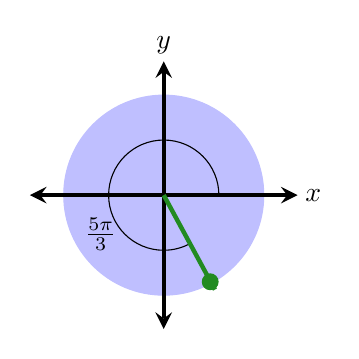
\begin{tikzpicture}
      % The main circle
      \draw[draw=blue!25!white,fill=blue!25!white] (0,0) circle (0.5in);

      % The x-y axis
      \draw (0,1.9) node[fill=white,anchor=center] {$y$};
      \draw (1.9,0) node[fill=white,anchor=center] {$x$};
      \draw[stealth-stealth,ultra thick] (0,1.7) -- (0,-1.7);
      \draw[stealth-stealth,ultra thick] (1.7,0) -- (-1.7,0);

      % Draw the angle arc
      \draw (0.7,0) arc[start angle=0,end angle=300,radius=0.7];
      \node at (-0.8,-0.5) {$\frac{5\pi}{3}$};
      \draw[ultra thick,ForestGreen] (0,0) -- (0.65,-1.2);
      \draw[ForestGreen,fill=ForestGreen] (0.59,-1.1) circle (0.1);
    \end{tikzpicture}

    \caption{}
  \end{figure}
\end{problem}

\begin{solution}
  \begin{align*}
    &\qquad P = \left(\cos \left(\frac{5\pi}{3}\right), \sin \left(\frac{5\pi}{3}\right)\right) \\
    \implies&\qquad P = \left(\frac{1}{2}, -\frac{\sqrt{3}}{2}\right) \\
  .\end{align*}

  Since we aren't on the \textbf{Unit Circle}, meaning we don't have a radius of
  $1$ units, we're going to scale up the length of the radius, which is $4$ 
  units.

  \[ P = \left(2, -2\sqrt{3}\right) \].
\end{solution}

\newpage

\begin{problem}
  Find the \textbf{exact} value for each of the following expressions. Be sure
  to use proper notation to communicate your answer, i.e., link the given
  expression and your answer with an equal sign. If the given expression is
  undefined write, \textit{"The expression is undefined."}

  \subparagraph{a.} $\cos (0)$

  \subparagraph{b.} $\sin (\frac{\pi}{6})$

  \subparagraph{c.} $\cos (\frac{5\pi}{4})$

  \subparagraph{d.} $\sin (\frac{4\pi}{3})$

  \subparagraph{e.} $\cos (-\frac{2\pi}{3})$

  \subparagraph{f.} $\sin (\frac{11\pi}{4})$

  \subparagraph{g.} $\tan (\pi)$

  \subparagraph{h.} $\sec (\frac{\pi}{2})$

  \subparagraph{i.} $\tan (\frac{11\pi}{6})$

  \subparagraph{j.} $\frac{10\pi}{3}$
\end{problem}

\begin{solution}
  \subparagraph{a.} $\cos (0) = 1$

  \subparagraph{b.} $\sin (\frac{\pi}{6}) = \frac{1}{2}$

  \subparagraph{c.} $\cos (\frac{5\pi}{4}) = -\frac{\sqrt{2}}{2}$

  \subparagraph{d.} $\sin (\frac{4\pi}{3}) = -\frac{\sqrt{3}}{2}$

  \subparagraph{e.} $\cos (-\frac{2\pi}{3}) = \frac{1}{2}$

  \subparagraph{f.} $\sin (\frac{11\pi}{4}) = \frac{\sqrt{2}}{2}$

  \subparagraph{g.} $\tan (\pi) = 0$

  \subparagraph{h.} $\sec (\frac{\pi}{2}) = $ \textit{The expression is undefined}

  \subparagraph{i.} $\tan (\frac{11\pi}{6}) = \sqrt{3}$

  \subparagraph{j.} $\csc (\frac{10\pi}{3}) = -\frac{2\sqrt{3}}{3}$
\end{solution}

\newpage

\begin{problem}
  Find the length of the arc spanned by an angle of $200^{\circ}$ in a circle of
  radius $12$ feet. [Provide a completely simplified, exact numerical value.]

  \begin{figure}[H]
    \centering
    \label{fig:4_units}

    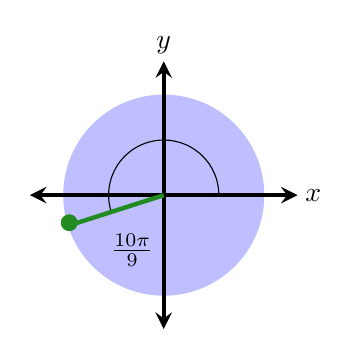
\begin{tikzpicture}
      % The main circle
      \draw[draw=blue!25!white,fill=blue!25!white] (0,0) circle (0.5in);

      % The x-y axis
      \draw (0,1.9) node[fill=white,anchor=center] {$y$};
      \draw (1.9,0) node[fill=white,anchor=center] {$x$};
      \draw[stealth-stealth,ultra thick] (0,1.7) -- (0,-1.7);
      \draw[stealth-stealth,ultra thick] (1.7,0) -- (-1.7,0);

      % Draw the angle arc
      \draw (0.7,0) arc[start angle=0,end angle=200,radius=0.7];
      \node at (-0.4,-0.7) {$\frac{10\pi}{9}$};
      \draw[ultra thick,ForestGreen] (0,0) -- (-1.25,-0.4);
      \draw[ForestGreen,fill=ForestGreen] (-1.2,-0.35) circle (0.1);
    \end{tikzpicture}

    \caption{}
  \end{figure}
\end{problem}

\begin{solution}
  To find the arc spanned by the angle, we can use the following formula:
  \[ s = r \times \theta \].
  Here's the catch. We cannot use degrees. We must convert $200^{\circ}$ to
  radians, which is pretty simple:
  \[ 200^{\circ} \times \frac{\pi}{180^{\circ}} = \frac{10\pi}{9} \].
  Now we can use the formula:
  \[ s = 12 \times \frac{10\pi}{9} = \frac{40\pi}{3} \].
  So, the arc spanned by the angle $200^{\circ}$ ($\frac{10\pi}{9}$ radians) is
  $\frac{40\pi}{3}$ feet.
\end{solution}

\newpage

\begin{problem}
  If $\sin (\theta) = \frac{\sqrt{7}}{5}$ and $\frac{\pi}{2} < \theta < \pi$,
  find the exact numerical values for the expressions given below. [Be sure to
  compose conclusions that directly communicate the values of the given
  expressions.]

  \subparagraph{a.} $\cos (\theta)$

  \subparagraph{b.} $\tan (\theta)$

  \subparagraph{c.} $\csc (\theta)$
\end{problem}

\begin{solution}
  \subparagraph{a.} $\cos (\theta)$

    \begin{align*}
      &\qquad \sin^{2} (\theta) = \cos^{2} (\theta) = 1 \\
      \implies&\qquad \left(\frac{\sqrt{7}}{5}\right)^{2} + \cos^{2} (\theta) = 1 \\
      \implies&\qquad \frac{7}{25} + \cos^{2} (\theta) = 1 \\
      \implies&\qquad \cos^{2} (\theta) = \frac{18}{25} \\
      \implies&\qquad \sqrt{\cos^{2}} (\theta) = \sqrt{\frac{18}{25}} \\
      \implies&\qquad \cos (\theta) = \frac{3\sqrt{2}}{5} \\
    .\end{align*}

  \subparagraph{b.} $\tan (\theta)$

    \begin{align*}
      &\qquad\tan \left(\theta\right) = \frac{\sin \left(\theta\right)}{\cos \left(\theta\right)} \\
      \implies&\qquad \tan (\theta) = \frac{\frac{\sqrt{7}}{5}}{\frac{3\sqrt{2}}{5}} \\
      \implies&\qquad\tan (\theta) = \frac{\sqrt{14}}{6} \\
    .\end{align*}

  \subparagraph{c.} $\csc (\theta)$

    \begin{align*}
      &\qquad\csc \left(\theta\right) = \frac{1}{\sin \left(\theta\right)} \\
      \implies&\qquad \csc(\theta) = \frac{1}{\frac{\sqrt{7}}{5}} \\
      \implies&\qquad \csc (\theta) = \frac{5}{\sqrt{7}} \\
      \implies&\qquad \csc (\theta) = \frac{5\sqrt{7}}{7} \\
    .\end{align*}
\end{solution}

\newpage

\begin{problem}
  Draw a graph of at least two period of the function $g(t) = 3\cos
  (\frac{\pi}{2}t + \frac{\pi}{2}) - 2$ by

  \begin{itemize}
    \item[(a)] plotting the points where the graph intersects the midline
    \item[(b)] plotting the points where the graph achieves maximum and minimum
      values
    \item[(c)] connecting these points with an appropriately curved sinusoidal
      wave.
  \end{itemize}

  \textbf{List the period, midline, and amplitude} of the function and
  \textbf{label the scale on the axes.}
\end{problem}

\begin{solution}
  \begin{figure}[htpb]
    \centering
    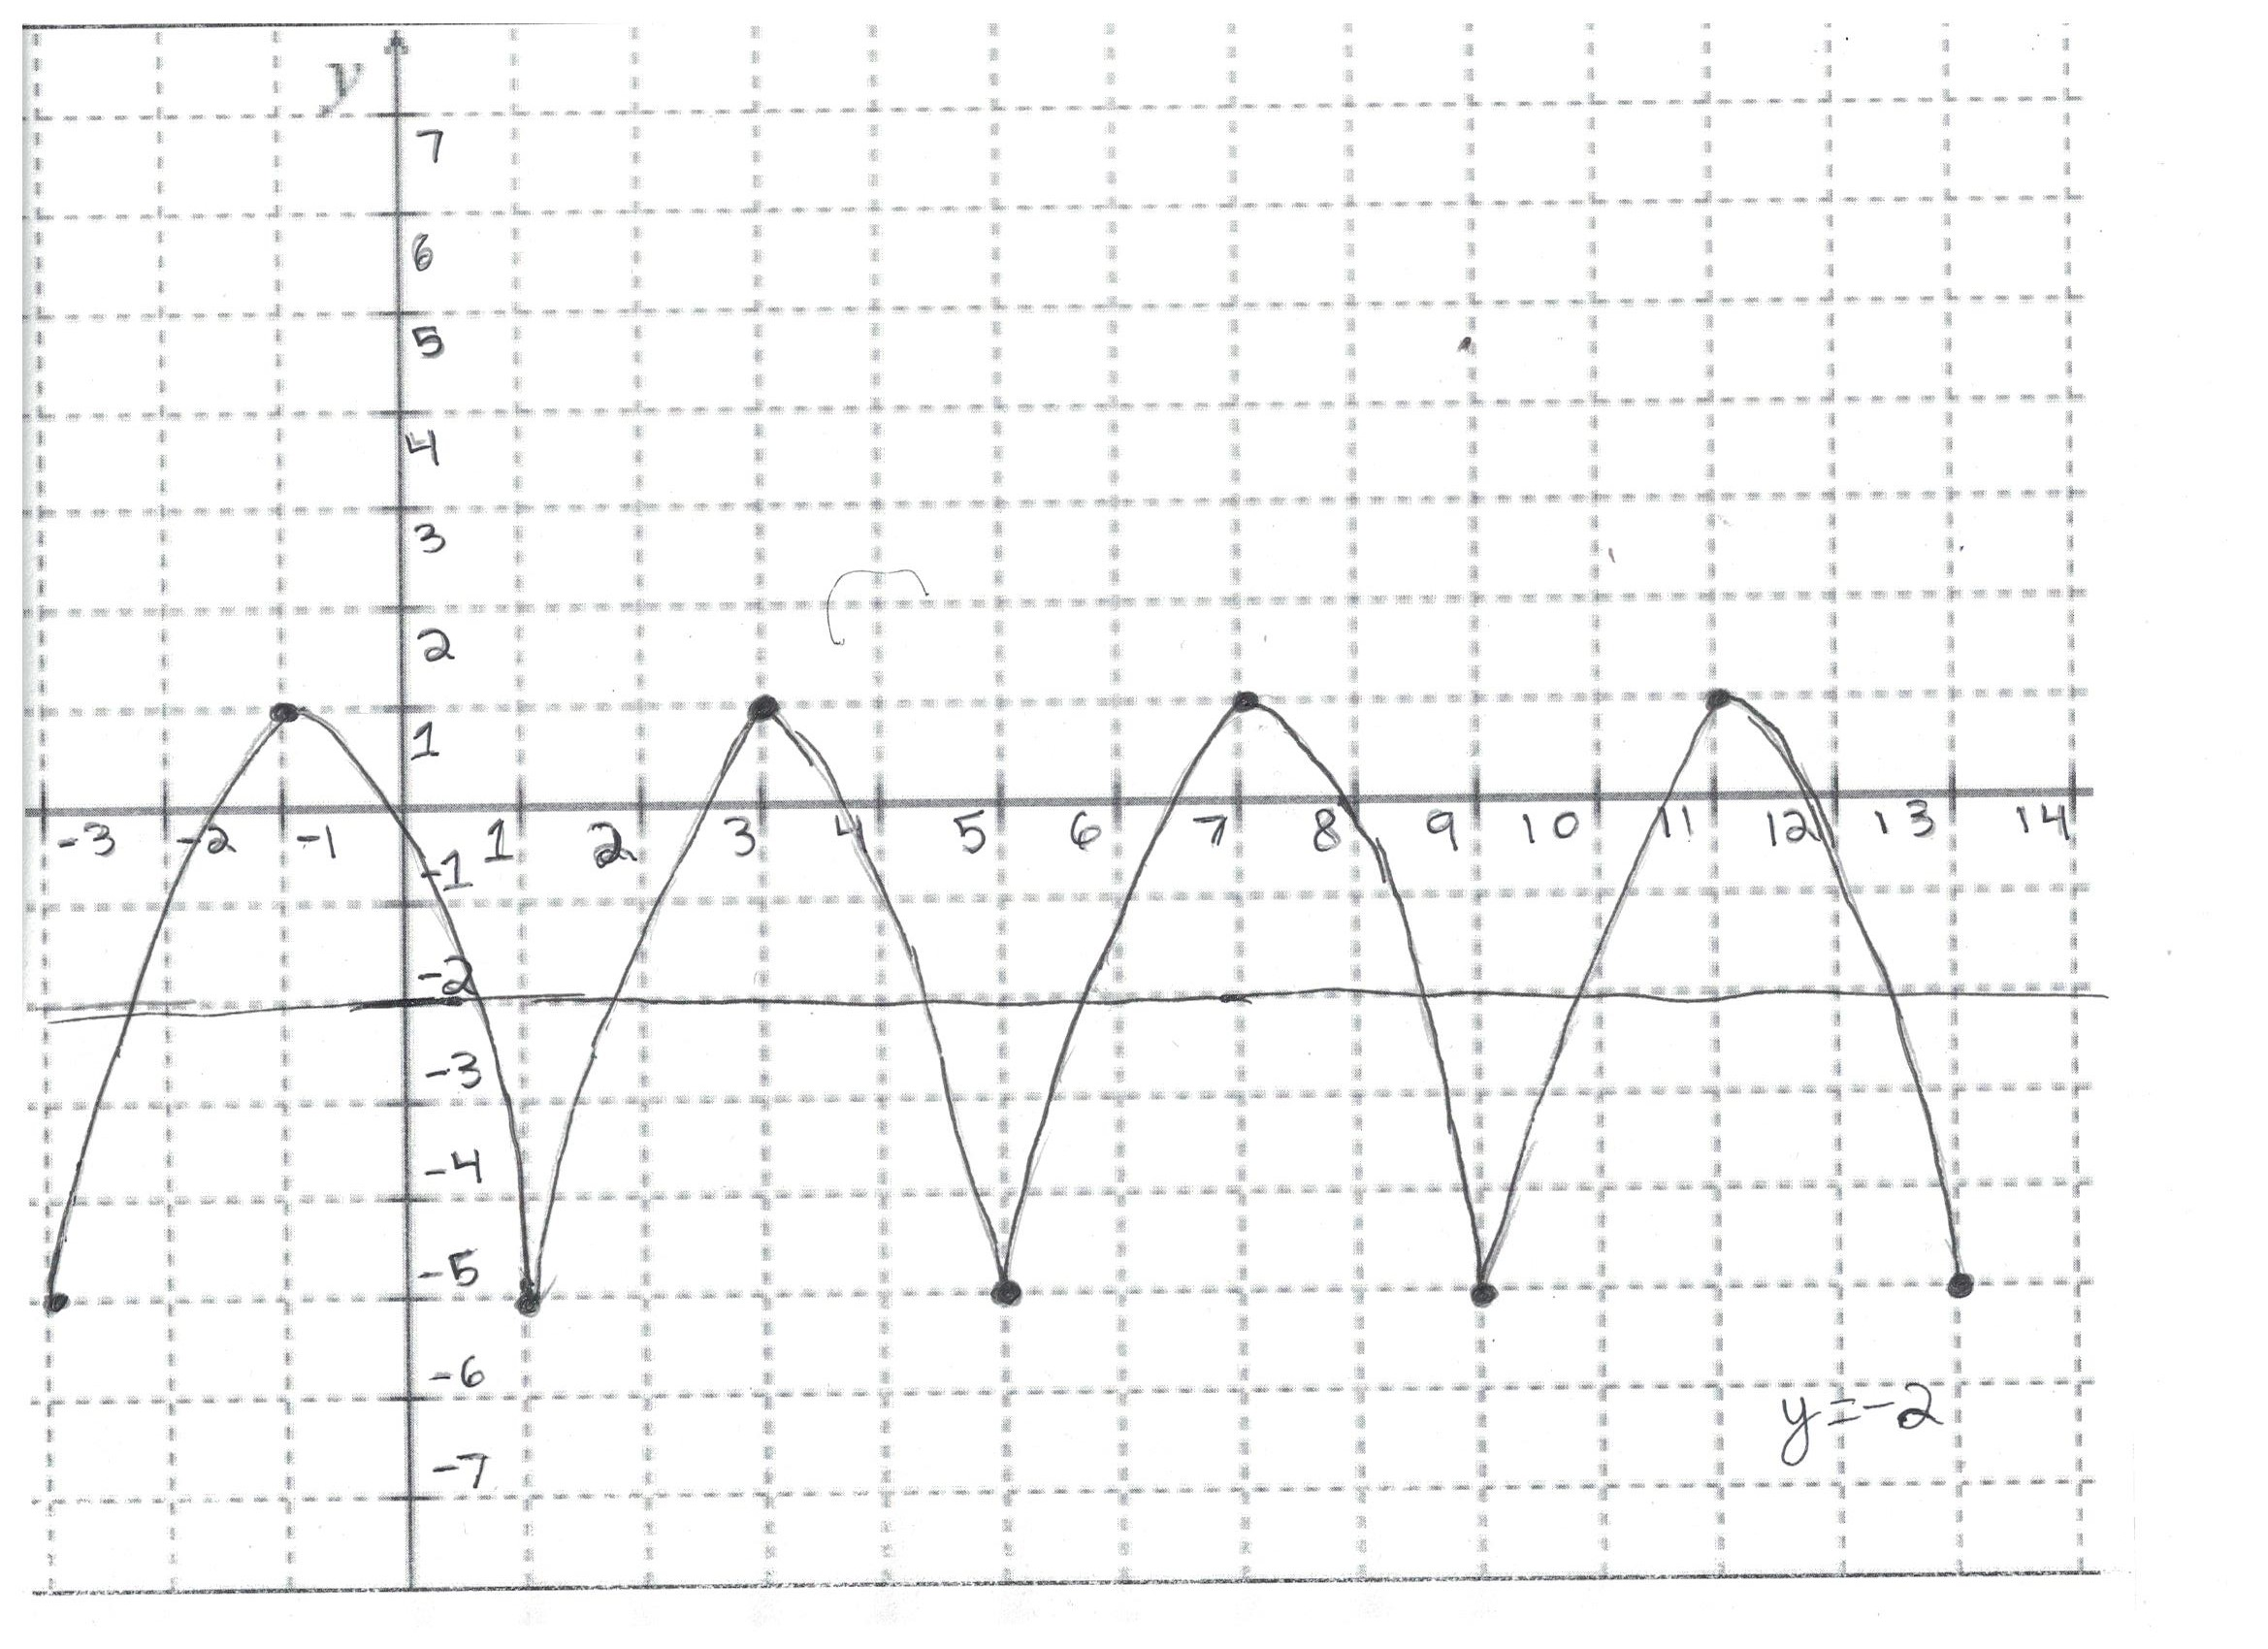
\includegraphics[width=0.8\textwidth]{images/midterm-a.png}
    \caption{Sketch a graph of $g(t) = 3\cos (\frac{\pi}{2}t + \frac{\pi}{2}) - 2$}
    \label{fig:graph_of_equation}
  \end{figure}
\end{solution}

\newpage

\begin{problem}
  Find a possible algebraic rule for the sinusoidal function $f$ graphed below.
  (You only need to provide one algebraic rule and you may utilize either the
  sin or cos function.)

  \begin{figure}[htpb]
    \centering
    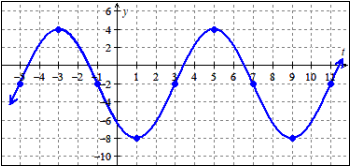
\includegraphics[width=0.8\textwidth]{images/midterm-b.png}
    \caption{The graph of $y = f(t)$}
    \label{fig:graph_of_equation}
  \end{figure}
\end{problem}

\begin{solution}
  To create an algebraic rule, we're going to use the following formula:

  \[ y = A\sin(\omega (t - h)) + k \textrm{ or } y = A\cos(\omega (t - h)) + k \].

  Where:

  \begin{enumerate}

    \item $A$ is the amplitude
    \item $\omega$ is the period
    \item $h$ is the horizontal shift
    \item $k$ is the midline
  \end{enumerate}

  Finding the amplitude is easy, but first we must find the midline. The midline
  for this graph is $-2$.
  To find the amplitude, we need to see how many units it takes to go from the
  maximum/minimum to the midline. In this case, that's $6$ units.
  Now I'm going to find the \textbf{period}, which is how long it takes to
  repeat itself. The period is $8$ units because it takes $8$ units to go from
  one maximum/minimum to the next. We only found the period. To find $\omega$,
  we know that sin and cos have a period of $2\pi$.

  \[ \frac{2\pi}{\omega} = 8 \implies \omega = \frac{\pi}{4} \].

  Since I'm using the sin function, $h = 3$.

  Here's our final algebraic rule:
  \[ y = -2 \left(\frac{\pi}{4} \left(t - 3\right)\right) - 2 \].
\end{solution}

\newpage

\begin{problem}
  Evaluate the following expressions. [Be sure to compose conclusions that
  directly communicate what the given expressions equal and to provide
  completely simplified exact numerical values.]

  \subparagraph{a.} $\sin (\cos^{-1} (-\frac{1}{2}))$

  \subparagraph{b.} $\cos^{-1} (\cos (\frac{7\pi}{6}))$
\end{problem}

\begin{solution}
  \subparagraph{a.} $\sin (\cos^{-1} (-\frac{1}{2}))$

    \begin{align*}
      &\qquad \sin \left(\cos^{-1} \left(-\frac{1}{2}\right)\right) \\
      \implies&\qquad\sin \left(\frac{2\pi}{3}\right) = \frac{\sqrt{3}}{2} \\
    .\end{align*}

  \subparagraph{b.} $\cos^{-1} (\cos (\frac{7\pi}{6}))$

    \begin{align*}
      &\qquad \cos^{-1} \left(\cos \left(\frac{7\pi}{6}\right)\right) = \frac{7\pi}{6} \\
    .\end{align*}
\end{solution}

\newpage

\begin{problem}
  Find \textbf{all} of the solutions of the following trigonometric equation.
  [Provide completely simplified, exact numerical values.]

  \[ 4\sin(2\theta) + 2 = 0 \].
\end{problem}

\begin{solution}
  \begin{align*} 
    &\qquad 4\sin(2\theta) + 2 = 0 \\
    \implies&\qquad 4\sin(2\theta) = -2 \\
    \implies&\qquad \sin(2\theta) = -\frac{1}{2} \\
    \implies&\qquad \sin^{-1} (\sin(2\theta)) = \sin^{-1} \left(-\frac{1}{2}\right) \\
    \implies&\qquad 2\theta = -\frac{\pi}{6} + 2k\pi \textrm{ or } 2\theta = \frac{7\pi}{6} + 2k\pi \\
    \implies&\qquad \frac{2\theta}{2} = \frac{-\frac{\pi}{6}}{2} + \frac{2k\pi}{2} \textrm{ or } \frac{2\theta}{2} = \frac{\frac{7\pi}{6}}{2} + \frac{2k\pi}{2} \\
    \implies&\qquad \theta = -\frac{\pi}{12} + k\pi \textrm{ or } \theta = \frac{7\pi}{12} + k\pi \forall k \in \mathbb{Z}
  .\end{align*}
\end{solution}

\newpage

\begin{problem}
  Find all the solutions of the following trigonometric equation
  \textbf{on the interval $[0, 2\pi]$}. [Provide completely simplified, exact
  numerical values.]

  \[ 6\sin(3x) + 4 = -2 \].
\end{problem}

\begin{solution}
  \begin{align*}
    &\qquad 6\sin(3x) + 4 = -2 \\
    \implies&\qquad 6\sin(3x) = -6 \\
    \implies&\qquad \frac{6\sin(3x)}{6} = -\frac{6}{6} \\
    \implies&\qquad \sin(3x) = -1 \\
    \implies&\qquad \sin^{-1} (\sin(3x)) = \sin^{-1} (-1) \\
    \implies&\qquad 3x = -\frac{\pi}{2} \\
    \implies&\qquad 3x = -\frac{\pi}{2} + 2k\pi \textrm{ or } 3x = \frac{3\pi}{2} + 2k\pi \\
    \implies&\qquad \frac{3x}{3} = \frac{-\frac{\pi}{2}}{3} + \frac{2k\pi}{3} \textrm{ or } \frac{3x}{3} = \frac{\frac{3\pi}{2}}{3} + \frac{2k\pi}{3} \\
    \implies&\qquad x = -\frac{\pi}{6} + \frac{2k\pi}{3} \textrm{ or } x = \frac{\pi}{2} + \frac{2k\pi}{3} \forall k \in \mathbb{Z}
  .\end{align*}
\end{solution}
